\chapter{Debugging and Profiling}
\label{ch:debugging}

\begin{chapterintro}
A slow job leaves evidence: in the SQL tab, the stages tab, the executor metrics,
the event log, and --- when you need it --- a flame graph. This chapter teaches you
to read that evidence in order, so that ``the job is slow'' becomes ``stage 2 has one
task nine times the median'' in a few minutes. Every failure it describes was
reproduced on purpose on the lab (\Cref{sec:refenv-lab}): a skewed join, three
different out-of-memory failures, a straggler with and without speculation, and a
stage that lost half its shuffle files. The numbers in each section are the real
output of those runs.
\end{chapterintro}

\section{The Spark UI as a diagnostic}
\label{sec:debug-ui}

The UI is organized as a funnel (\Cref{fig:ui-diagnostic-funnel}), and reading it in
the wrong order is the most common way to waste time on a slow job. The
\textbf{SQL} tab shows the physical plan with live metrics on every node, so you can
see \emph{which operator} is expensive before worrying about which stage or task.
The \textbf{Stages} tab is next: each stage's task-duration distribution is where
skew becomes visible as a gap between median and maximum. The \textbf{Executors} tab
aggregates across the application and shows imbalance between executors rather than
between tasks. Only once the operator and the stage are named does it pay to open
individual task metrics (\Cref{sec:reading-metrics}).

\begin{figure}[htbp]
  \centering
  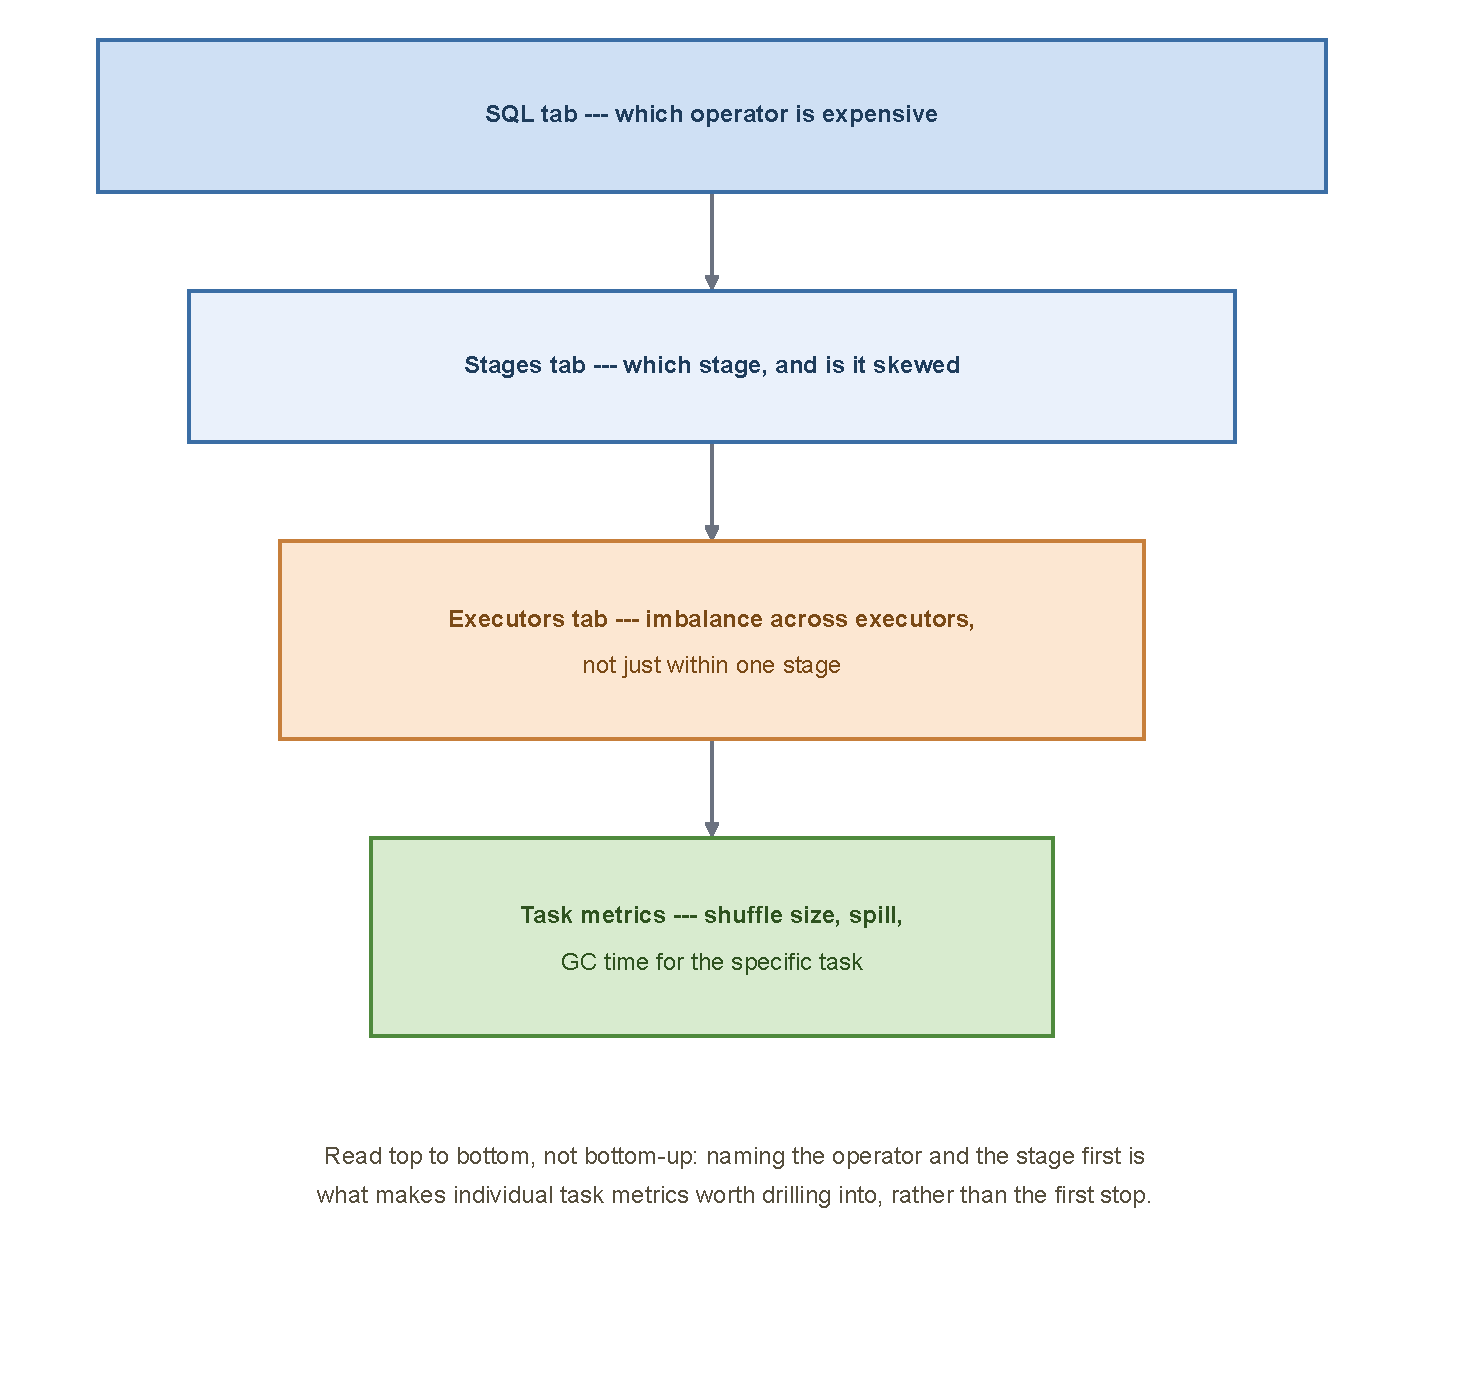
\includegraphics[width=\linewidth]{ui-diagnostic-funnel.pdf}
  \caption{The UI read top to bottom: each tab narrows the search before the next
  is worth opening.}
  \label{fig:ui-diagnostic-funnel}
\end{figure}

\section{Event logs and the history server}
\label{sec:debug-history}

Everything the live UI renders is first written to an \emph{event log}: a JSON-lines
file of every scheduler event, one line per event. The History Server replays that
file through the same listener objects that build the live UI, so by the last line
it holds the picture the live UI would have shown at exit --- which matters for the
jobs you most need to debug, those that failed and no longer have a UI. On
Kubernetes it is the only diagnostic that outlives the executor pods.

The lab opened one. A single join query (125 tasks over four stages) produced an
event log of 1.02~MB holding 276 events (\Cref{fig:eventlog-anatomy}).

\begin{figure}[htbp]
  \centering
  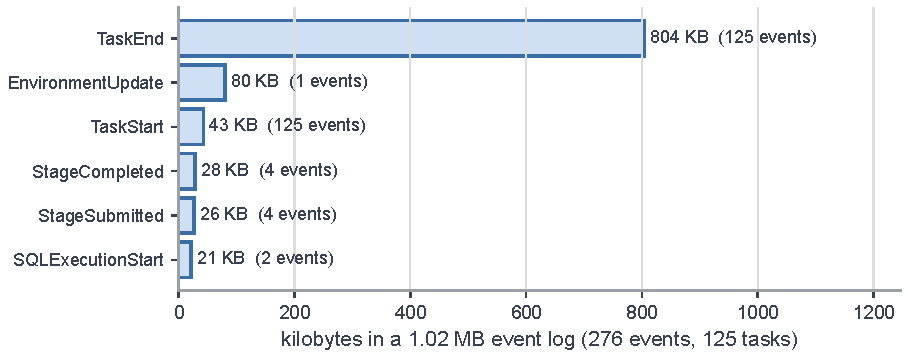
\includegraphics[width=\linewidth]{eventlog-anatomy.pdf}
  \caption{Bytes in the event log by event type. \texttt{TaskEnd} events, which carry
  every task's metrics, are 79\% of the file at about 6.4~KB each; the environment
  snapshot is the second-largest entry at 80~KB.}
  \label{fig:eventlog-anatomy}
\end{figure}

The size rule follows: an event log grows with the number of \emph{tasks}, about
6.4~KB per task here, so a job with 200,000 tasks writes about 1.3~GB, which is why
very large jobs need a log rolled over (\conf{spark.eventLog.rolling.enabled}) and
compressed (\conf{spark.eventLog.compress}) --- claim, from the documentation, not
tested in the lab.

\section{Reading task, shuffle, spill, and GC metrics}
\label{sec:reading-metrics}

A single task's detail is the finest-grained evidence the UI offers, and the lab
produced a real skewed stage to read. A sort-merge join of \texttt{orders} to
\texttt{dim\_product} on the hot product (30\% of the rows share one
\texttt{product\_id}), 40 shuffle partitions, a 1~GB heap and four cores, AQE off.
\Cref{fig:task-durations-skew} sorts the 40 tasks of the join stage by duration: 39
sit between 0.43 and 1.04~s and one takes 5.44~s.

\begin{figure}[htbp]
  \centering
  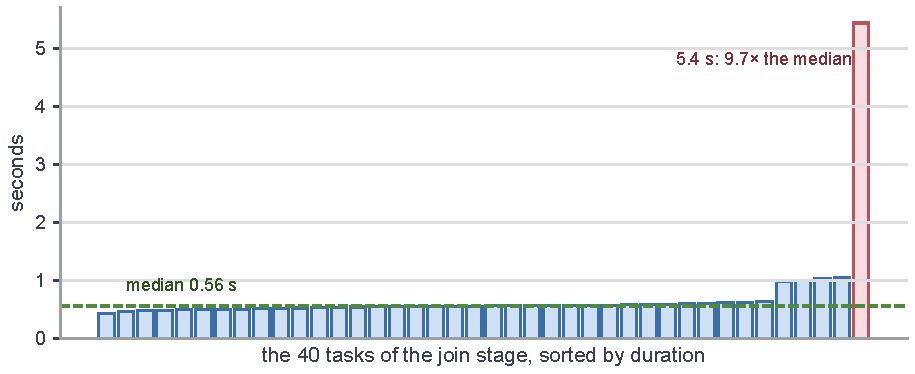
\includegraphics[width=\linewidth]{task-durations-skew.pdf}
  \caption{The 40 tasks of the join stage. One task is 9.7 times the median.}
  \label{fig:task-durations-skew}
\end{figure}

\Cref{fig:task-four-metrics} compares the median task with the slow one on the five
numbers that do the diagnostic work.

\begin{figure}[htbp]
  \centering
  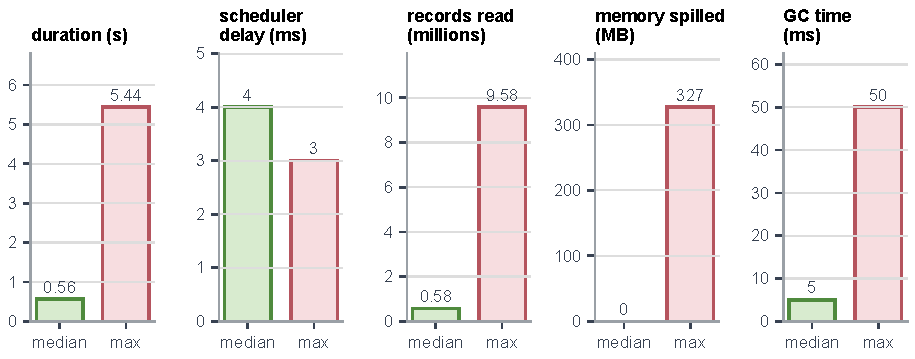
\includegraphics[width=\linewidth]{task-four-metrics.pdf}
  \caption{Median task against the slowest task of the same stage.}
  \label{fig:task-four-metrics}
\end{figure}

\begin{description}
  \item[Task duration against scheduler delay] separates real work from waiting for
        a slot. The slow task ran 5.44~s with a scheduler delay of 3~ms: all of it
        was work, not queueing, which rules out ``not enough slots'' and points at
        ``this task has too much to do.''
  \item[Records or bytes read in the same stage] is the most direct skew signal. The
        median task read 0.58~million records (8.2~MB); the slow one read 9.58
        million (82.2~MB) --- 16.5 times the records for 9.7 times the time.
  \item[Spill] appears when a task's share of execution memory was too small for its
        sort. Only the slow task spilled: 327~MB of memory spilled, 72~MB written
        to disk, where every other task spilled nothing (the share was 456~MB
        divided by 4 cores, \Cref{ch:tuning}).
  \item[GC time] was \emph{not} the story here: 50~ms of a 5.4~s task, about 1\%.
        A common narrative says skew drives GC; this measurement says check before
        assuming it, and that spill cost, not GC, was what the extra memory pressure
        bought.
\end{description}

Read together, the four numbers tell one story --- a task with 16 times the input
that spilled and ran ten times longer --- and it is the same cause
\Cref{sec:aqe-skew} detects and fixes automatically for a join, made visible here
for any stage.

\section{Common failure signatures}
\label{sec:failure-signatures}

A job rarely fails as one incomprehensible error. It fails as one of a small number
of recognizable signatures, each with its own evidence.

\paragraph{Out of memory: three failures, three traces.} The lab triggered each on
purpose (\Cref{tab:debug-oom}).

\begin{table}[htbp]
\centering\footnotesize
\renewcommand{\arraystretch}{1.25}
\begin{tabular}{@{}p{3.0cm}p{5.0cm}p{5.8cm}@{}}
\toprule
\textbf{How triggered} & \textbf{Evidence} & \textbf{What overflowed} \\
\midrule
\texttt{collect()} of 30~M rows, 512~MB heap & \texttt{java.lang.OutOfMemoryError: Java heap space}, logged as \texttt{Executor: Exception in task} & the JVM heap, by an allocation Spark does not track \\
\texttt{collect\_list} of one hot key, 512~MB heap & \texttt{SparkOutOfMemoryError: [UNABLE\_TO\_ACQUIRE\_MEMORY] Unable to acquire 65536 bytes of memory, got 0} & Spark's own execution-memory accounting: the pool had no 64~KB page to give \\
off-heap sort in a 1~GB container & exit code 137, \texttt{OOMKilled=true}, \textbf{zero} \texttt{OutOfMemoryError} lines in the log & the container's cgroup limit: heap plus off-heap exceeded what the kernel allowed \\
\bottomrule
\end{tabular}
\caption{Three OOM signatures, reproduced on the lab. The distinguishing evidence is
the exception class (or its absence), not the words ``out of memory.''}
\label{tab:debug-oom}
\end{table}

Two observations. First, the exception \emph{class} separates the first two:
\texttt{java.lang.OutOfMemoryError} is the JVM refusing an allocation;
\texttt{SparkOutOfMemoryError} is Spark's memory manager (\Cref{sec:mem-model})
refusing to grant a page, with the byte count it could not get. Second, in local
mode a driver \texttt{collect()} OOM was logged by an executor thread, because the
driver and executor share one JVM: on a cluster the same failure would appear in the
driver's log, and telling the two apart there is part of the diagnosis. The third
row has no exception at all, which is the signature --- the JVM never got a chance
to log, and the evidence is the container's exit status. Raising
\conf{spark.executor.memoryOverhead} is the fix for this one
(\Cref{sec:executor-sizing}), not the heap.

\paragraph{Stragglers and speculation.} A straggler is one task running far longer
than the rest with no data-size explanation, usually a node problem. The lab
simulated one: eight tasks of 3~s, with the first attempt of task 3 sleeping 40~s,
run on two workers registered under two different host names. Without speculation
the job took 41.3~s. With \conf{spark.speculation} on (multiplier 1.5, quantile
0.75) it took 11.2~s (\Cref{fig:speculation-gantt}): once six of eight tasks had
finished, Spark launched a copy of task 3 on a different executor at 8.1~s, which
finished 3.1~s later, and the original was killed.

\begin{figure}[htbp]
  \centering
  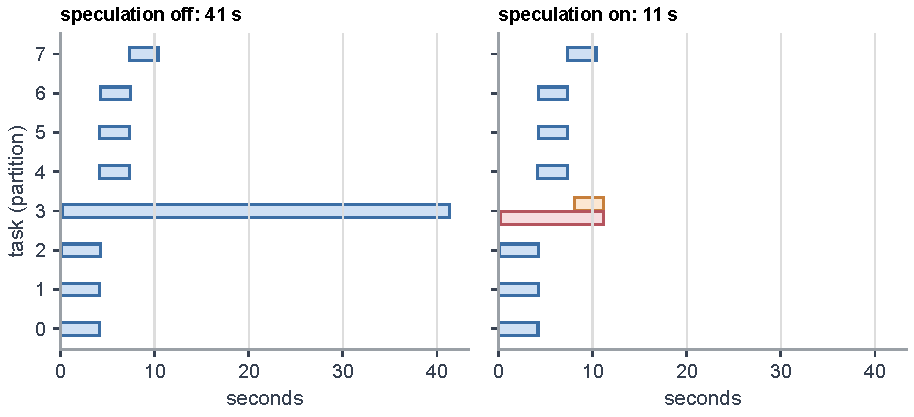
\includegraphics[width=\linewidth]{speculation-gantt.pdf}
  \caption{Task attempts without and with speculation. The speculative copy (orange)
  started at 8.1~s and won; the original (red) was killed when it did.}
  \label{fig:speculation-gantt}
\end{figure}

A detail that cost the lab one failed run: on a single worker with four executors all
on one host, speculation had no effect (41.6~s both ways). Spark does not place a
speculative copy on the host that already runs the original, so a cluster with one
host per executor pool cannot speculate. Speculation cuts tail latency for
node-related stragglers; for genuine skew it would just run the same oversized task
twice.

\paragraph{Fetch failures and stage retries.} Shuffle files are local to the
executor that wrote them, so losing the executor --- an OOM kill, a node drain,
dynamic allocation scaling down --- loses them. The lab reproduced the recovery:
after a job had run, it deleted 30 of the 57 shuffle files written by one of two
executors, then ran the same query again (\Cref{fig:fetch-failure-stages}).

\begin{figure}[htbp]
  \centering
  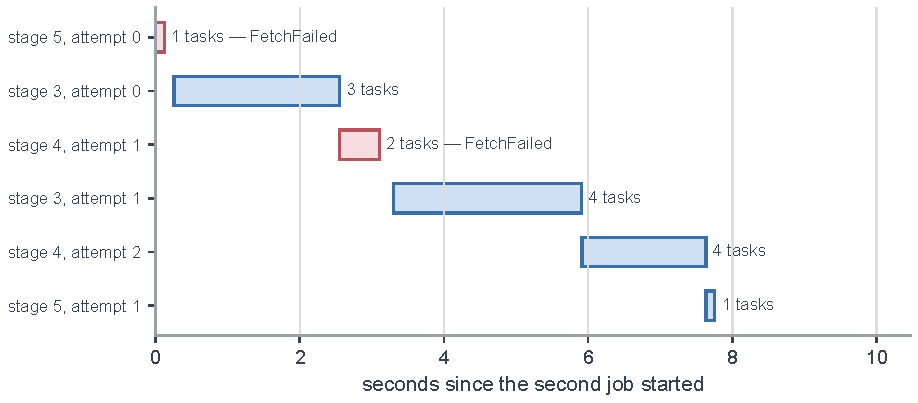
\includegraphics[width=\linewidth]{fetch-failure-stages.pdf}
  \caption{The stage attempts of the second run. The final stage failed at once with
  a \texttt{FetchFailedException}; the map stage re-ran for the missing output
  (3 tasks); a middle stage failed with a second \texttt{FetchFailedException}; the
  map stage ran again (4 tasks); then the middle and final stages succeeded. Three
  tasks failed with \texttt{FetchFailed}, 7.7~s in all.}
  \label{fig:fetch-failure-stages}
\end{figure}

A fetch failure is not a generic task failure. The scheduler recognizes it,
invalidates that executor's map outputs in the map output tracker
(\Cref{sec:sched-map-output-tracker}), and resubmits only the missing map tasks
before retrying the reduce stage. What the figure adds is that a stage chain can
fail in \emph{cascade}: the stage downstream of the lost output failed, and when
that recomputation reached a second exchange it hit missing files again. You see
this in the UI as stages with several attempts and a task count that varies by
attempt. Two layers retry, and tuning the wrong one does nothing: the shuffle
client retries a fetch from a live executor (\conf{spark.shuffle.io.maxRetries},
\conf{spark.shuffle.io.retryWait}); a genuinely lost executor is handled by stage
resubmission, bounded by \conf{spark.stage.maxConsecutiveAttempts} (4) and
\conf{spark.task.maxFailures} (4). Raise both on a cluster where executors are
routinely reclaimed.

\section{async-profiler and flame graphs}
\label{sec:debug-profiler}

The UI's metrics answer \emph{which stage and which task}; they do not answer
\emph{which method is burning CPU} in a task that is neither spilling nor GC-bound.
Instrumenting profilers rewrite every method to time it, so their overhead scales
with call frequency. \texttt{async-profiler} samples instead: it interrupts the JVM
at a fixed interval and reads the call stacks, so the cost is fixed per interrupt
and independent of how hot the code is. The fraction of samples in a method
converges on the fraction of time it consumes, and a flame graph draws exactly that:
one bar per stack frame, width proportional to samples. A wide bar under a
Spark-internal frame usually means the bottleneck is in a UDF or expression the
generated code calls (\Cref{ch:tungsten}, where a Python UDF cost 32 times a
built-in), not in Spark's execution machinery. (Claim --- not exercised in the
lab, which has no profiler installed: the sampling mechanism and its low overhead
are as documented by the project.)

\section{Debugging query plans}
\label{sec:debug-plans}

A plan that does not do what you expect is diagnosed the way \Cref{ch:catalyst}
taught you to read one, applied adversarially: compare the \emph{analyzed} plan
with what you intended (a wrong join condition or an implicit cast shows up here);
check the \emph{optimized} plan for whether pushdown and pruning fired
(\Cref{fig:pushdown-rows-by-predicate} is the catalogue of what defeats them); and
compare the \emph{physical} plan's joins and exchanges with what \Cref{ch:joins} and
\Cref{ch:shuffle} predict. \texttt{EXPLAIN FORMATTED}'s numbered node list plus
per-node detail is almost always more useful than the tree alone, because you can
cross-reference a node's exact filters and build side. A hint that appears ignored
is checked the same way: read the operator (\Cref{sec:joins-measured}).

\section{From symptom to lever}
\label{sec:debug-levers}

\begin{table}[htbp]
\centering\footnotesize
\renewcommand{\arraystretch}{1.25}
\begin{tabular}{@{}p{3.1cm}p{3.9cm}p{4.0cm}p{3.1cm}@{}}
\toprule
\textbf{Symptom} & \textbf{Evidence} & \textbf{Lever} & \textbf{Cost} \\
\midrule
one task far slower than the rest & max/median duration 9.7$\times$; records read 16$\times$ & skew handling (\Cref{ch:aqe}) or repartition by a better key & shuffle cost \\
one slow task, ordinary input & records read near the median; scheduler delay low & \conf{spark.speculation} (and only if node-related) & duplicate compute; needs more than one host \\
\texttt{java.lang.OutOfMemoryError} & exception class names the JVM heap & raise executor heap, or shrink what the task holds & memory per executor \\
\texttt{SparkOutOfMemoryError} & ``Unable to acquire \dots\ got 0'' & raise unified pool per task: more heap or fewer cores (\Cref{fig:spill-vs-share}) & memory, or slots \\
executor vanishes, no exception & exit code 137, \texttt{OOMKilled} & raise \conf{spark.executor.memoryOverhead} & pod size \\
stage runs several times & \texttt{FetchFailedException}, attempts $>$ 1 & shuffle service, tracking timeout, retries (\Cref{ch:tuning}) & held executors \\
event log is huge & about 6.4~KB per task & roll and compress the log & history-server CPU \\
\bottomrule
\end{tabular}
\caption{The debugging levers: symptom, evidence, lever, cost.}
\label{tab:debug-levers}
\end{table}

\section{Summary}
\label{sec:debug-summary}

Diagnose top-down: the SQL tab names the expensive operator, the Stages tab names the
stage and shows skew as a task-duration outlier, and only then do individual task
metrics confirm the mechanism. In the lab's skewed stage one task read 16.5 times the
records, spilled while its 39 neighbours did not, and took 9.7 times as long, with GC
at 1\% --- a reminder to read the numbers before telling the textbook story. The event
log makes this possible after the job has exited and costs about 6.4~KB per task. Three
OOM failures leave three different traces, told apart by the exception class or its
absence. A straggler on a separate host is cut from 41.3 to 11.2~s by speculation,
which cannot act on a single host. A lost executor's shuffle files trigger a cascade
of stage attempts, not a single retry.

\exercisehead
\begin{exercises}
\item Take a stage summary of your own and compute the max-to-median ratio of
      duration and of records read. If the ratios differ by a large factor, what does
      that say about the cause?
\item Trigger each of the three OOM signatures on a test cluster and record the
      exception class (or the absence of one) and the exit status.
\item Reproduce \Cref{fig:fetch-failure-stages} by deleting one executor's shuffle
      files between two runs of the same DataFrame, then count the stage attempts and
      \texttt{FetchFailed} tasks in the event log.
\end{exercises}
